\documentclass{beamer}

\usetheme{CambridgeUS}
\usecolortheme{orchid}

\usepackage[utf8]{inputenc}
\usepackage[T1]{fontenc}

% Math
\usepackage{amsmath}
\usepackage{amssymb}
\usepackage{bm}

% Graphics
\usepackage{graphicx}
\usepackage{caption}
\usepackage{subcaption}
\graphicspath{{../figs/}}

% Colors
\definecolor{darkblue}{HTML}{00688B}
\definecolor{darkgreen}{HTML}{6E8B3D}
\definecolor{cadet}{HTML}{DAE1FF}
\definecolor{salmon}{HTML}{FFB08A}

% Listings
\usepackage{textcomp}
\usepackage{listings}
\lstset{
  keywordstyle=\bfseries\color{orange},
  stringstyle=\color{darkblue!80},
  commentstyle=\color{darkblue!80},
  showstringspaces=false,
  basicstyle=\ttfamily,
  upquote=true,
}
\lstdefinestyle{fortran}{
  language=Fortran,
  morekeywords={for},
  deletekeywords={status},
}
\lstdefinestyle{c}{
  language=C,
  morekeywords={include},
}
\lstdefinestyle{shell}{
  language=bash,
}

\subtitle{TMA4280---Introduction to Supercomputing}

\begin{document}


\title{Message passing and MPI}
\author{Eivind Fonn}
\institute{SINTEF ICT / NTNU}
\date{December 2015}
\maketitle

\begin{frame}
  \frametitle{The message passing model}
  \begin{center}
    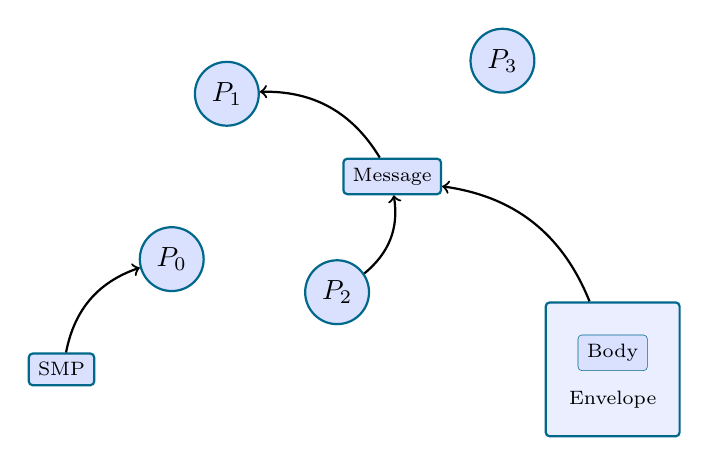
\begin{tikzpicture}[
  proc/.style={shape=circle, draw=darkblue, fill=cadet, thick},
  msg/.style={shape=rectangle, draw=darkblue, fill=cadet, thick, rounded corners=0.5mm},
  env/.style={minimum height=1.7cm, minimum width=1.7cm},
  scale=0.7,
  ]
  \node[proc] (p0) at (0,0) {$P_0$};
  \node[proc] (p1) at (1,3) {$P_1$};
  \node[proc] (p2) at (3,-0.6) {$P_2$};
  \node[proc] (p3) at (6,3.6) {$P_3$};
  \node[msg] (msg) at (4.0, 1.5) {\scriptsize Message};
  \node[msg, env, fill=cadet!55] (env) at (8, -2.0) {};
  \node[msg, very thin] (body) at (8, -1.7) {\scriptsize Body};
  \node[below of=body, node distance=6mm] {\scriptsize Envelope};
  \draw[->, thick] (p2) edge[bend right] node [right] {} (msg);
  \draw[->, thick] (msg) edge[bend right] node [right] {} (p1);
  \draw[->, thick] (env) edge[bend right] node [right] {} (msg);

  \node[msg] (smp) at (-2,-2) {\scriptsize SMP};
  \draw[->, thick] (smp) edge[bend left] node [right] {} (p0);
\end{tikzpicture}

  \end{center}
\end{frame}

\begin{frame}[fragile]
  \frametitle{MPI with C}
  \scalebox{0.5}{
    \lstinputlisting[style=c]{\code/mpi_hello/c/hello.c}
  }
\end{frame}

\begin{frame}[fragile]
  \frametitle{MPI with Fortran}
  \scalebox{0.5}{
    \lstinputlisting[style=fortran]{\code/mpi_hello/fortran/hello.f90}
  }
\end{frame}

\begin{frame}[fragile]
  \frametitle{Sample output with four processors}
  \begin{center}
    \begin{tabular}{c}
\begin{lstlisting}
Process 0: Hello, world!
Process 1: Hello, world!
Process 3: Hello, world!
Process 2: Hello, world!
\end{lstlisting}
    \end{tabular}
  \end{center}
  Note that ordering is not guaranteed.
\end{frame}

\begin{frame}
  \frametitle{MPI: Message Passing Interface}
  Advantages of the MPI message-passing model:
  \begin{itemize}
  \item standardization;
  \item portability;
  \item performance;
  \item expressiveness.
  \end{itemize}

  MPI is a library comprising about 125 functions or operations:
  \begin{itemize}
  \item \textcolor{red}{one-to-one} operations (or point-to-point communication);
  \item \textcolor{red}{one-to-all} operations;
  \item \textcolor{red}{all-to-one} operations;
  \item \textcolor{red}{all-to-all} operations.
  \end{itemize}
  The last three types are referred to as {\em collective} operations.
\end{frame}

\begin{frame}[fragile]
  \frametitle{Header file}
  The header file is required. For C:
\begin{lstlisting}[style=c]
#include "mpi.h"
\end{lstlisting}

  And for Fortran:
\begin{lstlisting}[style=fortran]
include 'mpif.h'
\end{lstlisting}
\end{frame}

\begin{frame}[fragile]
  \frametitle{Calling functions}
  For C:
\begin{lstlisting}[style=c,morekeywords={err}]
err = MPI_Xxxxx(parameters, ...);
\end{lstlisting}
  Or ignoring the error code:
\begin{lstlisting}[style=c,morekeywords={err}]
MPI_Xxxxx(parameters, ...);
\end{lstlisting}

  For Fortran, everything is a subroutine:
\begin{lstlisting}[style=fortran,morekeywords={err}]
call MPI_XXXXX(parameters, ..., err)
\end{lstlisting}
\end{frame}

\begin{frame}
  \frametitle{Six essential functions}
  \begin{center}
    \bgroup\def\arraystretch{1.2}
    \addtolength{\tabcolsep}{0.5cm}
    \begin{tabular}{ll}
      \hline
      C & Fortran  \\
      \hhline{==}
      \texttt{MPI\_Init} & \texttt{call MPI\_Init} \\
      \texttt{MPI\_Comm\_size} & \texttt{call MPI\_Comm\_size} \\
      \texttt{MPI\_Comm\_rank} & \texttt{call MPI\_Comm\_rank} \\
      \texttt{MPI\_Send} & \texttt{call MPI\_Send} \\
      \texttt{MPI\_Recv} & \texttt{call MPI\_Recv} \\
      \texttt{MPI\_Finalize} & \texttt{call MPI\_Finalize} \\
      \hline
    \end{tabular}
    \addtolength{\tabcolsep}{-0.5cm}
    \egroup
  \end{center}
\end{frame}

\begin{frame}
  \frametitle{Message = data + envelope}
  \texttt{\textcolor{red}{MPI\_Send}($\underbrace{buffer, count, datatype}_{\textcolor{blue}{data}}$,
    $\underbrace{dest, tag, comm}_{\textcolor{blue}{envelope}}$); } \\
  \texttt{\textcolor{red}{MPI\_Recv}($\underbrace{buffer, count, datatype}_{\textcolor{blue}{data}}$,
    $\underbrace{source, tag, comm,\&status}_{\textcolor{blue}{envelope}}$); }

  Examples of predefined data types (C):
  \begin{itemize}
  \item \texttt{MPI\_CHAR}
  \item \texttt{MPI\_INT}
  \item \texttt{MPI\_FLOAT}
  \item \texttt{MPI\_DOUBLE}
  \end{itemize}
\end{frame}

\begin{frame}[fragile]
  \frametitle{Point-to-point communication}
  \texttt{MPI\_Send} and \texttt{MPI\_Recv} are \emph{blocking}. Deadlock
  example:
  \begin{center}
    \begin{tabular}{c}
\begin{lstlisting}[style=c,morekeywords={MPI_Recv,MPI_Send}]
if (rank == 0) {
  MPI_Recv(...);
  MPI_Send(...);
}
else if (rank == 1) {
  MPI_Recv(...);
  MPI_Send(...);
}
\end{lstlisting}
    \end{tabular}
  \end{center}
\end{frame}

\begin{frame}[fragile]
  \frametitle{Point-to-point communication}
  How to avoid deadlock.
  \begin{center}
    \begin{tabular}{c}
\begin{lstlisting}[style=c,morekeywords={MPI_Recv,MPI_Send}]
if (rank == 0) {
  MPI_Send(...);
  MPI_Recv(...);
}
else if (rank == 1) {
  MPI_Recv(...);
  MPI_Send(...);
}
\end{lstlisting}
    \end{tabular}
  \end{center}
\end{frame}

\begin{frame}[fragile]
  \frametitle{Collective operations}
  In general,
  \begin{itemize}
  \item Involves all of the processes in a group, and
  \item are more efficient and less tedious to use compared to point-to-point
    communication.
  \end{itemize}
  An example (synchronization between processes):
  \begin{center}
    \begin{tabular}{c}
\begin{lstlisting}[style=c,morekeywords={MPI_Barrier}]
MPI_Barrier(comm);
\end{lstlisting}
    \end{tabular}
  \end{center}
\end{frame}

\begin{frame}
  \frametitle{Collective operations}
  \begin{center}
    \begin{tikzpicture}[scale=0.6]
      \foreach \i in {0,...,4} {
        \foreach \j in {0,9} {
          \foreach \k in {0,6} {
            \draw[darkblue, thick] (\i+\j,0+\k) -- (\i+\j,4+\k);
            \draw[darkblue, thick] (0+\j,\i+\k) -- (4+\j,\i+\k);
          }
        }
      }
      \node at (0.5,9.5) {$A_0$};
      \node at (9.5,9.5) {$A_0$};
      \node at (9.5,8.5) {$A_0$};
      \node at (9.5,7.5) {$A_0$};
      \node at (9.5,6.5) {$A_0$};

      \node at (0.5,3.5) {$A_0$};
      \node at (0.5,2.5) {$A_1$};
      \node at (0.5,1.5) {$A_2$};
      \node at (0.5,0.5) {$A_3$};
      \node at (9.5,3.5) {$A_0$};
      \node at (10.5,3.5) {$A_1$};
      \node at (11.5,3.5) {$A_2$};
      \node at (12.5,3.5) {$A_3$};
      \node[color=black!30] at (9.5,2.5) {$A_1$};
      \node[color=black!30] at (9.5,1.5) {$A_2$};
      \node[color=black!30] at (9.5,0.5) {$A_3$};

      \draw[red, very thick, ->] (4.5,8) -- (8.5,8);
      \draw[red, very thick, ->] (4.5,2) -- (8.5,2);
      \node[anchor=north] at (6.5,8) {\texttt{MPI\_Bcast}};
      \node[anchor=south] at (6.5,8) {\scriptsize One-to-all broadcast};
      \node[anchor=north] at (6.5,2) {\texttt{MPI\_Gather}};
      \node[anchor=south] at (6.5,2) {\scriptsize All-to-one gather};

      \node[anchor=west, color=darkblue] (data) at (0,10.5) {\scriptsize Data};
      \node[anchor=west, color=darkblue, rotate=-90] (procs) at (-0.5,10) {\scriptsize Processes};
      \draw[darkblue, ->] (data.east) -- ($ (data.east) + (1.5,0) $);
      \draw[darkblue, ->] (procs.east) -- ($ (procs.east) - (0,1.5) $);
    \end{tikzpicture}
  \end{center}
\end{frame}

\begin{frame}
  \frametitle{Global reduction}
  \begin{center}
    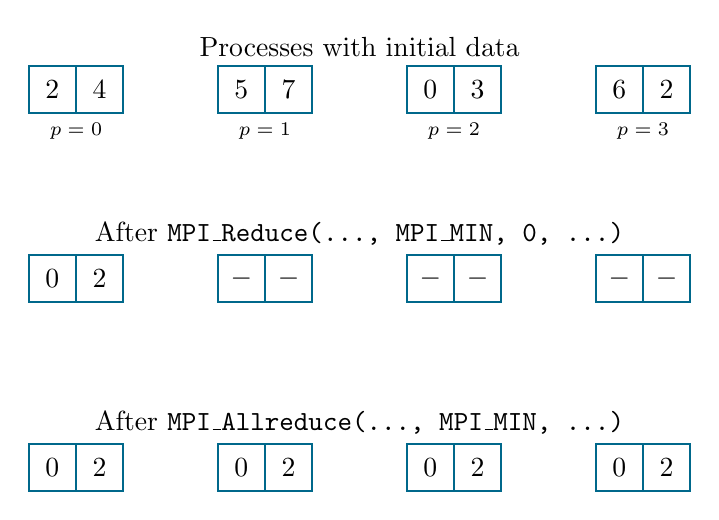
\begin{tikzpicture}[scale=0.6]
      \foreach \i in {0,4,8,12} {
        \foreach \j in {0,4,8} {
          \draw[darkblue, thick] (\i,\j) rectangle (\i+2,\j+1);
          \draw[darkblue, thin] (\i+1,\j) -- (\i+1,\j+1);
        }
      }

      \node[anchor=south] at (7,9) {Processes with initial data};
      \node[anchor=north] at (1,8) {\scriptsize $p=0$};
      \node[anchor=north] at (5,8) {\scriptsize $p=1$};
      \node[anchor=north] at (9,8) {\scriptsize $p=2$};
      \node[anchor=north] at (13,8) {\scriptsize $p=3$};
      \node at (0.5,8.5) {$2$}; \node at (1.5,8.5) {$4$};
      \node at (4.5,8.5) {$5$}; \node at (5.5,8.5) {$7$};
      \node at (8.5,8.5) {$0$}; \node at (9.5,8.5) {$3$};
      \node at (12.5,8.5) {$6$}; \node at (13.5,8.5) {$2$};

      \node[anchor=south] at (7,5) {After \texttt{MPI\_Reduce(..., MPI\_MIN, 0, ...)}};
      \node at (0.5,4.5) {$0$}; \node at (1.5,4.5) {$2$};
      \node at (4.5,4.5) {$-$}; \node at (5.5,4.5) {$-$};
      \node at (8.5,4.5) {$-$}; \node at (9.5,4.5) {$-$};
      \node at (12.5,4.5) {$-$}; \node at (13.5,4.5) {$-$};

      \node[anchor=south] at (7,1) {After \texttt{MPI\_Allreduce(..., MPI\_MIN, ...)}};
      \node at (0.5,0.5) {$0$}; \node at (1.5,0.5) {$2$};
      \node at (4.5,0.5) {$0$}; \node at (5.5,0.5) {$2$};
      \node at (8.5,0.5) {$0$}; \node at (9.5,0.5) {$2$};
      \node at (12.5,0.5) {$0$}; \node at (13.5,0.5) {$2$};
    \end{tikzpicture}
  \end{center}
\end{frame}

\begin{frame}
  \frametitle{Global reduction}
  \texttt{\textcolor{red}{MPI\_Reduce}($\underbrace{sbuf, rbuf, count, datatype}_{\textcolor{blue}{data}}$,
    $\underbrace{op, root, comm}_{\textcolor{blue}{envelope}}$); } \\
  \texttt{\textcolor{red}{MPI\_Allreduce}($\underbrace{sbuf, rbuf, count, datatype}_{\textcolor{blue}{data}}$,
    $\underbrace{op, comm}_{\textcolor{blue}{envelope}}$); }

  Examples of predefined operations (C):
  \begin{itemize}
  \item \texttt{MPI\_SUM}
  \item \texttt{MPI\_PROD}
  \item \texttt{MPI\_MIN}
  \item \texttt{MPI\_MAX}
  \end{itemize}
\end{frame}

\begin{frame}
  \frametitle{A ``problem'': defining $\pi$ through integration}
  \begin{align*}
    & \int_0^1\frac{1}{1+x^2} \dif{x} \\
    &= [\arctan(x)]_0^1 \\
    &= \arctan(1) - \arctan(0) = \frac{\pi}{4}
  \end{align*}
  Hence,
  \begin{align*}
    \pi = \int_0^1\frac{4}{1+x^2} \dif{x}
  \end{align*}
\end{frame}

\begin{frame}
  \frametitle{Numerical integration}
  \begin{center}
    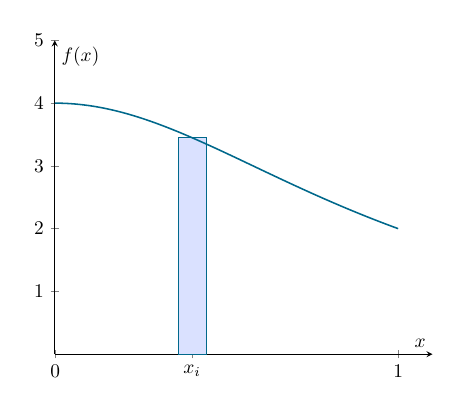
\begin{tikzpicture}[scale=0.7]
      \begin{axis}[
        xmin=0,
        xmax=1.1,
        ymin=0,
        ymax=5,
        axis lines=middle,
        xlabel={$x$},
        ylabel={$f(x)$},
        xtick={0.001,0.4,1},
        xticklabels={$0$, $x_i$, $1$},
        ]
        \draw[darkblue, fill=cadet] (axis cs:0.36,0) rectangle (axis cs:0.44,3.4482);
        \addplot[darkblue, thick, domain=0:1, samples=100]{4/(1+x^2)};
      \end{axis}
    \end{tikzpicture}
  \end{center}
  \[
    A_i = \left ( \frac{4}{1+x_i^2} \right ) \cdot h, \qquad
    \text{with} \quad x_i = \left (i+\frac{1}{2} \right )\cdot h
  \]
  where $i=0,\ldots,n-1$, and $h=1/n$.
\end{frame}

\begin{frame}
  \frametitle{Numerical integration}
  \begin{align*}
    \pi = \int_0^4 \frac{4}{1 + x^2} \dif{x} \approx
    h \sum_{i=0}^{n-1} \frac{4}{1 + x_i^2} = \pi_n
  \end{align*}
\end{frame}

\begin{frame}[fragile]
  \frametitle{Calculating pi with MPI in C}
  \begin{center}
    \begin{tabular}{c}
      \scalebox{0.65}{
      \lstinputlisting
      [style=c, firstline=1, lastline=22, morekeywords={
      MPI_Init, MPI_Comm_size, MPI_Comm_rank, MPI_Wtime}]{\code/pi/pi.c}
      }
    \end{tabular}
  \end{center}
\end{frame}

\begin{frame}[fragile]
  \frametitle{Calculating pi with MPI in C (cntd.)}
  \begin{center}
    \begin{tabular}{c}
      \scalebox{0.65}{
      \lstinputlisting
      [style=c, firstline=24, lastline=45, morekeywords={
      MPI_Reduce, MPI_Finalize, MPI_Wtime}]{\code/pi/pi.c}
      }
    \end{tabular}
  \end{center}
\end{frame}

\begin{frame}
  \frametitle{Things to consider}
  \begin{enumerate}
  \item Is the program correct, e.g., is the convergence rate as expected?
  \item Is the program load-balanced?
  \item Do we get the same value of $\pi_n$ for different values of $P$?
  \item Is the program scalable?
  \end{enumerate}
\end{frame}

\begin{frame}
  \frametitle{Convergence test}
  \begin{center}
    \bgroup\def\arraystretch{1.2}
    \begin{tabular}{cc}
      \hline
      $n$ & $\text{error} = |\pi - \pi_n |$
      \\ \hhline{==} 10 & $8.33\cdot 10^{-4}$
      \\ \hline $10^2$ & $8.33\cdot 10^{-6}$
      \\ \hline $10^3$ & $8.33\cdot 10^{-8}$
      \\ \hline $10^4$ & $8.33\cdot 10^{-10}$
      \\ \hline $10^5$ & $8.37\cdot 10^{-12}$
      \\ \hline
    \end{tabular}
    \egroup
  \end{center}
  Hence, $|\pi - \pi_n | \sim {\cal O}(h^2)$ where $h = 1/n$.
\end{frame}

\begin{frame}
  \frametitle{Scalability: timing results on Vilje}
  \begin{center}
    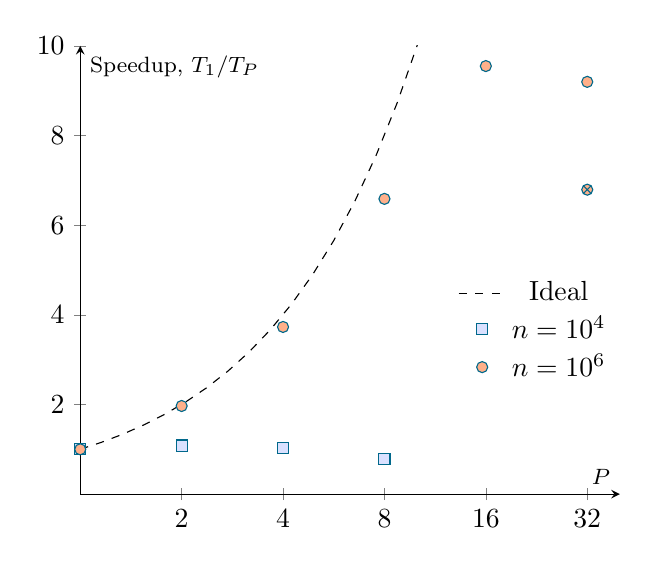
\begin{tikzpicture}
      \begin{axis}[
        xmin=1,
        xmax=40,
        ymin=0,
        ymax=10,
        axis lines=middle,
        xlabel={{\footnotesize $P$}},
        ylabel={{\footnotesize Speedup, $T_1/T_P$}},
        xtick={1,2,4,8,16,32},
        xticklabels={1,2,4,8,16,32},
        xmode=log,
        legend style={
          at={(1,0.50)},
          draw=none,
        }
        ]
        \addplot[domain=1:32, dashed] {x};
        \addplot[only marks, draw=darkblue, fill=cadet, mark=square*]
        coordinates {(1,1) (2,1.083) (4,1.020) (8,0.782)};
        \addplot[only marks, draw=darkblue, fill=salmon, mark=*]
        coordinates {(1,1) (2,1.966) (4,3.729) (8,6.586) (16,9.548) (32,9.196)};
        \addplot[only marks, draw=darkblue, fill=salmon, mark=otimes*] coordinates {(32,6.791)};
        \legend{Ideal, $n=10^4$, $n=10^6$}
      \end{axis}
    \end{tikzpicture}
  \end{center}
\end{frame}

\begin{frame}
  \frametitle{Inner product}
  \begin{align*}
    \sigma = \bm x^\intercal \bm y = \bm x \cdot \bm y = \sum_{m=0}^{M-1} x_m y_m
  \end{align*}
  \begin{center}
    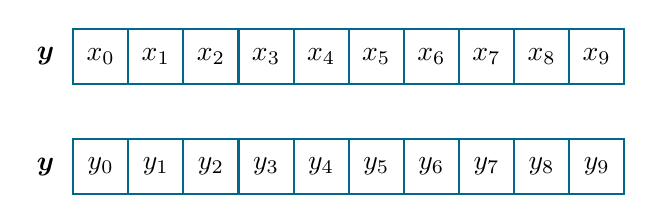
\begin{tikzpicture}[scale=0.7]
      \foreach \i in {0,...,9} {
        \node at (\i+0.5,2.5) {$x_\i$};
        \node at (\i+0.5,0.5) {$y_\i$};
        \draw[darkblue, thick] (\i,0) rectangle (\i+1,1);
        \draw[darkblue, thick] (\i,2) rectangle (\i+1,3);
      }
      \node at (-0.5,0.5) {$\bm y$};
      \node at (-0.5,2.5) {$\bm y$};
    \end{tikzpicture}
  \end{center}
\end{frame}

\begin{frame}
  \frametitle{Distribution of work}
  \begin{center}
    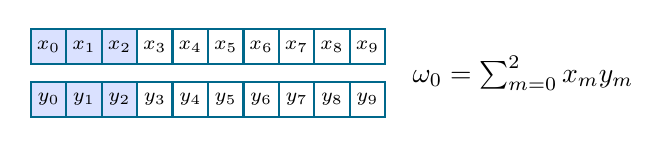
\begin{tikzpicture}[scale=0.45]
      \foreach \i in {0,...,2} {
        \draw[darkblue, fill=cadet, thick] (\i,0) rectangle (\i+1,1);
        \draw[darkblue, fill=cadet, thick] (\i,1.5) rectangle (\i+1,2.5);
      }
      \foreach \i in {3,...,9} {
        \draw[darkblue, thick] (\i,0) rectangle (\i+1,1);
        \draw[darkblue, thick] (\i,1.5) rectangle (\i+1,2.5);
      }
      \foreach \i in {0,...,9} {
        \node at (\i+0.5,2.0) {${\scriptstyle x_\i}$};
        \node at (\i+0.5,0.5) {${\scriptstyle y_\i}$};
      }
      \node[anchor=west] at (10.5,1.25) {$\omega_0 = \sum_{m=0}^2 x_m y_m$};
    \end{tikzpicture}
    \\~\\
    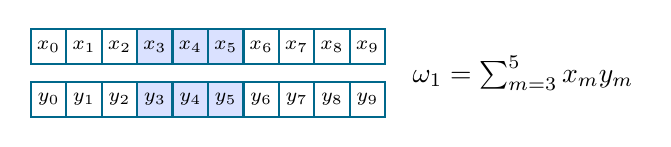
\begin{tikzpicture}[scale=0.45]
      \foreach \i in {3,4,5} {
        \draw[darkblue, fill=cadet, thick] (\i,0) rectangle (\i+1,1);
        \draw[darkblue, fill=cadet, thick] (\i,1.5) rectangle (\i+1,2.5);
      }
      \foreach \i in {0,1,2,6,7,8,9} {
        \draw[darkblue, thick] (\i,0) rectangle (\i+1,1);
        \draw[darkblue, thick] (\i,1.5) rectangle (\i+1,2.5);
      }
      \foreach \i in {0,...,9} {
        \node at (\i+0.5,2.0) {${\scriptstyle x_\i}$};
        \node at (\i+0.5,0.5) {${\scriptstyle y_\i}$};
      }
      \node[anchor=west] at (10.5,1.25) {$\omega_1 = \sum_{m=3}^5 x_m y_m$};
    \end{tikzpicture}
    \\~\\
    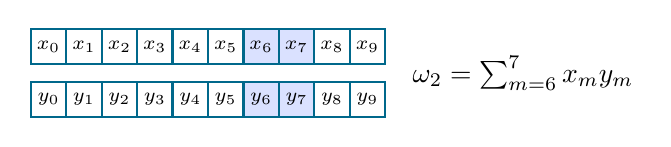
\begin{tikzpicture}[scale=0.45]
      \foreach \i in {6,7} {
        \draw[darkblue, fill=cadet, thick] (\i,0) rectangle (\i+1,1);
        \draw[darkblue, fill=cadet, thick] (\i,1.5) rectangle (\i+1,2.5);
      }
      \foreach \i in {0,1,2,3,4,5,8,9} {
        \draw[darkblue, thick] (\i,0) rectangle (\i+1,1);
        \draw[darkblue, thick] (\i,1.5) rectangle (\i+1,2.5);
      }
      \foreach \i in {0,...,9} {
        \node at (\i+0.5,2.0) {${\scriptstyle x_\i}$};
        \node at (\i+0.5,0.5) {${\scriptstyle y_\i}$};
      }
      \node[anchor=west] at (10.5,1.25) {$\omega_2 = \sum_{m=6}^7 x_m y_m$};
    \end{tikzpicture}
    \\~\\
    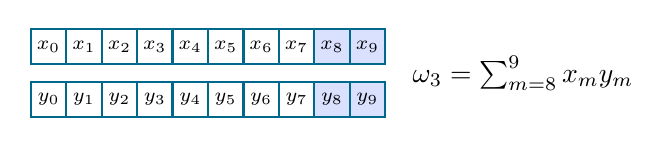
\begin{tikzpicture}[scale=0.45]
      \foreach \i in {8,9} {
        \draw[darkblue, fill=cadet, thick] (\i,0) rectangle (\i+1,1);
        \draw[darkblue, fill=cadet, thick] (\i,1.5) rectangle (\i+1,2.5);
      }
      \foreach \i in {0,...,7} {
        \draw[darkblue, thick] (\i,0) rectangle (\i+1,1);
        \draw[darkblue, thick] (\i,1.5) rectangle (\i+1,2.5);
      }
      \foreach \i in {0,...,9} {
        \node at (\i+0.5,2.0) {${\scriptstyle x_\i}$};
        \node at (\i+0.5,0.5) {${\scriptstyle y_\i}$};
      }
      \node[anchor=west] at (10.5,1.25) {$\omega_3 = \sum_{m=8}^9 x_m y_m$};
    \end{tikzpicture}
  \end{center}
\end{frame}

\begin{frame}
  \frametitle{Program on processor $p$}
  \begin{align*}
    \bm x, \bm y &: \text{ vectors of dimension } M \\
    \omega_p &= \sum_{m \in \mathcal{M}_p} x_m y_m \\
                 & \text{Send } \omega_p  \text{ to processor } q \not= p \\
                 & \text{Receive } \omega_q  \text{ from processor } q \\
    \sigma &= \sum_{q=0}^{P-1} \omega_q.
  \end{align*}
\end{frame}

\begin{frame}
  \frametitle{Local and global numbering}
  Global indices: $\mathcal{M} = \{0,1,2,\ldots,M-1\}$.
  Cardinality $|\mathcal{M}| = M$.

  Subdivision:
  \begin{align*}
    \mathcal{M} = \bigcup_{p=0}^{P-1} \mathcal{M}_p, \qquad
    \mathcal{M}_p \cap \mathcal{M}_q = \emptyset, \qquad
    p \not= q.
  \end{align*}

  \begin{itemize}
  \item $\mathcal{M}_p$: a subset of global indices
  \item $M_p = |\mathcal{M}_p|$: the number of global indices assigned to
    process $p$.
  \item $\mathcal{I}_p = \{0,1,\ldots,M_p-1\}$: a \emph{local} index set
  \end{itemize}

  Note $|\mathcal{I}_p| = |\mathcal{M}_p| = M_p$.
\end{frame}

\begin{frame}
  \frametitle{Local and global numbering}
  \begin{center}
    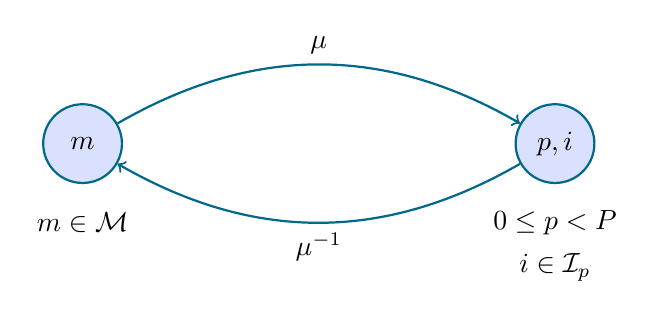
\begin{tikzpicture}
      \node[circle, thick, fill=cadet, draw=darkblue, minimum size=1cm] (g) at (-3,0) {$m$};
      \node[circle, thick, fill=cadet, draw=darkblue, minimum size=1cm] (l) at (3,0) {$p,i$};
      \draw[->, draw=darkblue, thick] (g) edge[bend left] node [above] {$\mu$} (l);
      \draw[->, draw=darkblue, thick] (l) edge[bend left] node [below] {$\mu^{-1}$} (g);
      \node at (-3,-1) {$m\in\mathcal{M}$};
      \node (p) at (3,-1) {$0 \leq p < P$};
      \node[anchor=north] at (p.south) {$i \in \mathcal{I}_p$};
    \end{tikzpicture}
  \end{center}
\end{frame}

\begin{frame}
  \frametitle{Distribution of work and data}
  \begin{center}
    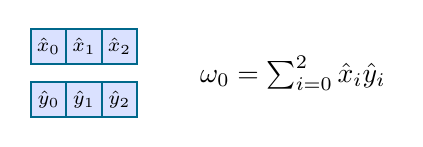
\begin{tikzpicture}[scale=0.45]
      \foreach \i in {0,1,2} {
        \draw[darkblue, fill=cadet, thick] (\i,0) rectangle (\i+1,1);
        \draw[darkblue, fill=cadet, thick] (\i,1.5) rectangle (\i+1,2.5);
        \node at (\i+0.5,2.0) {${\scriptstyle \hat{x}_\i}$};
        \node at (\i+0.5,0.5) {${\scriptstyle \hat{y}_\i}$};
      }
      \node[anchor=west] at (4.5,1.25) {$\omega_0 = \sum_{i=0}^2 \hat{x}_i \hat{y}_i$};
    \end{tikzpicture}
    \\~\\
    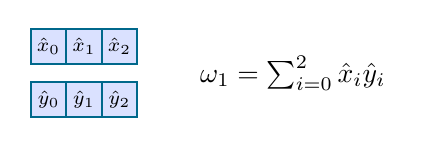
\begin{tikzpicture}[scale=0.45]
      \foreach \i in {0,1,2} {
        \draw[darkblue, fill=cadet, thick] (\i,0) rectangle (\i+1,1);
        \draw[darkblue, fill=cadet, thick] (\i,1.5) rectangle (\i+1,2.5);
        \node at (\i+0.5,2.0) {${\scriptstyle \hat{x}_\i}$};
        \node at (\i+0.5,0.5) {${\scriptstyle \hat{y}_\i}$};
      }
      \node[anchor=west] at (4.5,1.25) {$\omega_1 = \sum_{i=0}^2 \hat{x}_i \hat{y}_i$};
    \end{tikzpicture}
    \\~\\
    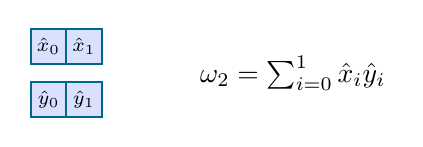
\begin{tikzpicture}[scale=0.45]
      \foreach \i in {0,1} {
        \draw[darkblue, fill=cadet, thick] (\i,0) rectangle (\i+1,1);
        \draw[darkblue, fill=cadet, thick] (\i,1.5) rectangle (\i+1,2.5);
        \node at (\i+0.5,2.0) {${\scriptstyle \hat{x}_\i}$};
        \node at (\i+0.5,0.5) {${\scriptstyle \hat{y}_\i}$};
      }
      \node[anchor=west] at (4.5,1.25) {$\omega_2 = \sum_{i=0}^1 \hat{x}_i \hat{y}_i$};
    \end{tikzpicture}
    \\~\\
    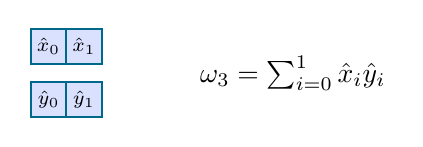
\begin{tikzpicture}[scale=0.45]
      \foreach \i in {0,1} {
        \draw[darkblue, fill=cadet, thick] (\i,0) rectangle (\i+1,1);
        \draw[darkblue, fill=cadet, thick] (\i,1.5) rectangle (\i+1,2.5);
        \node at (\i+0.5,2.0) {${\scriptstyle \hat{x}_\i}$};
        \node at (\i+0.5,0.5) {${\scriptstyle \hat{y}_\i}$};
      }
      \node[anchor=west] at (4.5,1.25) {$\omega_3 = \sum_{i=0}^1 \hat{x}_i \hat{y}_i$};
    \end{tikzpicture}
  \end{center}
\end{frame}

\begin{frame}
  \frametitle{Program on processor $p$}
  \begin{align*}
    \hat{\bm x}, \hat{\bm y} &: \text{ vectors of dimension } I_p \\
    \omega_p &= \sum_{i=0}^{I_p-1} \hat{x}_i \hat{y}_i
    = \sum_{i=0}^{I_p-1} x_{\mu^{-1}(p,i)} y_{\mu^{-1}(p,i)}
    = \sum_{m \in \mathcal{M}_p} x_m y_m. \\
                 & \text{Send } \omega_p  \text{ to processor } q \not= p \\
                 & \text{Receive } \omega_q  \text{ from processor } q \\
    \sigma &= \sum_{q=0}^{P-1} \omega_q.
  \end{align*}
\end{frame}

\begin{frame}
  \frametitle{Global reduction}
  Reduction algorithm for the global sum
  \[
    \sigma = \sum_{q=0}^{P-1} \omega_q.
  \]
  \texttt{\textcolor{red}{MPI\_Reduce}(}$\omega$, $\sigma$,
  \texttt{1, MPI\_DOUBLE, MPI\_SUM, 0, MPI\_COMM\_WORLD)} \\
  (the answer will be known to process zero), or \\~\\
  \texttt{\textcolor{red}{MPI\_Allreduce}(}$\omega$, $\sigma$,
  \texttt{1, MPI\_DOUBLE, MPI\_SUM, MPI\_COMM\_WORLD)}
  (the answer will be known to every process)
\end{frame}

\begin{frame}
  \frametitle{Global sum $P=4$, \texttt{MPI\_Reduce}}
  \begin{center}
    \begin{tikzpicture}[scale=0.7]
      \node (a0) at (0,3) {$p=0: \quad \omega_0$};
      \node (a1) at (0,2) {$p=1: \quad \omega_1$};
      \node (a2) at (0,1) {$p=2: \quad \omega_2$};
      \node (a3) at (0,0) {$p=3: \quad \omega_3$};

      \node[right=1 of a0] (b0) {$\omega_0 + \omega_1$};
      \node[right=1 of a2] (b2) {$\omega_2 + \omega_3$};

      \node[right=1 of b0] (c0) {$\omega_0 + \omega_1 + \omega_2 + \omega_3 = \sigma$};

      \draw[thick, darkblue, ->] (a1.east) -- (b0.west);
      \draw[thick, darkblue, ->] (a3.east) -- (b2.west);
      \draw[thick, darkblue, ->] (b2.east) -- (c0.west);
    \end{tikzpicture}
  \end{center}
  Can be completed in $\log_2 P$ steps.
\end{frame}

\begin{frame}
  \frametitle{Global sum $P=4$, \texttt{MPI\_Allreduce}}
  \begin{center}
    \begin{tikzpicture}[scale=0.7]
      \node (a0) at (0,3) {$p=0: \quad \omega_0$};
      \node (a1) at (0,2) {$p=1: \quad \omega_1$};
      \node (a2) at (0,1) {$p=2: \quad \omega_2$};
      \node (a3) at (0,0) {$p=3: \quad \omega_3$};

      \node[right=1 of a0] (b0) {$\omega_0 + \omega_1$};
      \node[right=1 of a1] (b1) {$\omega_1 + \omega_0$};
      \node[right=1 of a2] (b2) {$\omega_2 + \omega_3$};
      \node[right=1 of a3] (b3) {$\omega_3 + \omega_2$};

      \node[right=1 of b0] (c0) {$\omega_0 + \omega_1 + \omega_2 + \omega_3 = \sigma$};
      \node[right=1 of b1] (c1) {$\omega_1 + \omega_0 + \omega_3 + \omega_2 = \sigma$};
      \node[right=1 of b2] (c2) {$\omega_2 + \omega_3 + \omega_0 + \omega_1 = \sigma$};
      \node[right=1 of b3] (c3) {$\omega_3 + \omega_2 + \omega_1 + \omega_0 = \sigma$};

      \draw[thick, darkblue, ->] (a0.east) -- (b1.west);
      \draw[thick, darkblue, ->] (a1.east) -- (b0.west);
      \draw[thick, darkblue, ->] (a2.east) -- (b3.west);
      \draw[thick, darkblue, ->] (a3.east) -- (b2.west);
      \draw[thick, darkblue, ->] (b0.east) -- (c2.west);
      \draw[thick, darkblue, ->] (b1.east) -- (c3.west);
      \draw[thick, darkblue, ->] (b2.east) -- (c0.west);
      \draw[thick, darkblue, ->] (b3.east) -- (c1.west);
    \end{tikzpicture}
  \end{center}
  Can be completed in $\log_2 P$ steps.
\end{frame}

\begin{frame}
  \frametitle{Program on processor $p$}
  \begin{align*}
    \hat{\bm x}, \hat{\bm y} &: \text{ vectors of dimension } I_p \\
    \sigma &= \sum_{i=0}^{I_p-1} \hat{x}_i \hat{y}_i
             = \sum_{i=0}^{I_p-1} x_{\mu^{-1}(p,i)} y_{\mu^{-1}(p,i)}
             = \sum_{m \in \mathcal{M}_p} x_m y_m. \\
                             & \text{for } d=0,\ldots,\log_2 P - 1 \\
    & \quad \text{Send } \sigma \text{ to processor } q = p \;\overline{\vee}\; 2^d \\
    & \quad \text{Receive } \sigma_q \text{ from processor } q = p \;\overline{\vee}\; 2^d \\
    & \quad \sigma = \sigma + \sigma_q \\
    & \text{end}
  \end{align*}
  Here, $\overline{\vee}$ is exclusive or. $p$ and $p\;\overline{\vee}\;2^d$
  differ only in bit $d$.
\end{frame}

\input{postamble}
